\documentclass[11pt]{article}
\usepackage[T1]{fontenc}
\usepackage[margin=1in]{geometry}
\usepackage{amsmath,amssymb,array,booktabs,graphicx}
\usepackage{placeins}
\usepackage[hidelinks]{hyperref}
\setlength{\floatsep}{8pt plus 2pt minus 2pt}
\setlength{\textfloatsep}{10pt plus 2pt minus 3pt}
\newcommand{\HoneVerdict}{inconclusive}
\newcommand{\HtwoVerdict}{unsupported}
\newcommand{\SampleStart}{1926-07-01}
\newcommand{\SampleEnd}{2026-09-30}
\newcommand{\TestStart}{1970-01-01}
\newcommand{\EstimationStart}{1926-07-01}
\newcommand{\EstimationEnd}{1949-12-31}
\newcommand{\CalibrationStart}{1950-01-01}
\newcommand{\CalibrationEnd}{1969-12-31}
\newcommand{\EventClusters}{21}
\newcommand{\AnchorCount}{10793}
\newcommand{\SelectedLambda}{0.998}
\newcommand{\VarianceFloor}{1e-08}
\newcommand{\LogChiMean}{-1.27}
\newcommand{\ObservationVariance}{4.935}
\newcommand{\UKFAlpha}{0.5}
\newcommand{\UKFBeta}{2}
\newcommand{\UKFKappa}{0}
\newcommand{\RidgePrior}{10}
\newcommand{\PrimaryHorizon}{5}
\newcommand{\SecondaryHorizon}{20}
\newcommand{\RotationLag}{20}
\newcommand{\SubspaceRank}{3}
\newcommand{\VolWindow}{20}
\newcommand{\CorrelationWindow}{60}
\newcommand{\CovarianceWindow}{250}
\newcommand{\PeakWindow}{250}
\newcommand{\AnnualizationDays}{252}
\newcommand{\StandardFloor}{0.05}
\newcommand{\StandardClip}{6}
\newcommand{\EventThreshold}{-15\%}
\newcommand{\MergeDays}{120}
\newcommand{\ForecastDays}{60}
\newcommand{\LogisticC}{1}
\newcommand{\PurgeDays}{60}
\newcommand{\RefitDays}{252}
\newcommand{\BootstrapBlock}{250}
\newcommand{\SurrogateBlock}{60}
\newcommand{\MinimumSurrogateP}{0.002}
\newcommand{\SupportThreshold}{0.02}
\newcommand{\AttemptCount}{5}
\newcommand{\UKFError}{1.24e-14}
\newcommand{\FiniteDifferenceError}{9.77e-11}
\newcommand{\EOnePassCount}{10}
\newcommand{\GOneRelativeError}{0.03818}
\newcommand{\GOneOffDiagonalCorrelation}{0.8608}
\newcommand{\GTwoRotationContrast}{0.2618}
\newcommand{\GTwoAmplificationContrast}{2.312}
\newcommand{\GThreeImprovement}{59.27\%}
\newcommand{\GFourMedianRho}{0.988}
\newcommand{\GFourMedianF}{1.071}
\newcommand{\GFourMaximumF}{1.329}
\newcommand{\GFourDirectGap}{0.08337}
\newcommand{\DeltaMZero}{-0.01366}
\newcommand{\DeltaMZeroLow}{-0.02799}
\newcommand{\DeltaMZeroHigh}{0.001076}
\newcommand{\DeltaMOne}{-0.008816}
\newcommand{\DeltaMOneLow}{-0.02427}
\newcommand{\DeltaMOneHigh}{0.004163}
\newcommand{\HTwoPZero}{0.088}
\newcommand{\HTwoPOne}{0.17}
\newcommand{\HoneAdjpR}{0.844}
\newcommand{\HoneAdjpH}{0.984}
\newcommand{\HoneAdjpF}{0.006}
\newcommand{\HoneEventAdjpR}{1}
\newcommand{\HoneEventAdjpH}{1}
\newcommand{\HoneEventAdjpF}{1}
\newcommand{\HoneEventRawpR}{0.3846}
\newcommand{\HoneEventRawpH}{0.8142}
\newcommand{\HoneEventRawpF}{0.8252}
\newcommand{\MaxSpearman}{0.4793}
\newcommand{\PCANinetyComponents}{4}
\newcommand{\DirectionPercentile}{5.9\%}
\newcommand{\DirectionDateCount}{14308}
\newcommand{\WedinShare}{2.5\%}
\newcommand{\SurrogateThreshold}{0.01}
\newcommand{\EventPlaceboThreshold}{0.05}
\newcommand{\HoneUnsupportedRule}{all adjusted block-shuffle probabilities are at least the pre-onset placebo threshold}
\newcommand{\DirectionInterpretation}{The covariance and susceptibility spaces are more closely aligned than most Haar reference subspaces}
\newcommand{\DirectionVarianceText}{more closely aligned than most Haar reference subspaces}
\newcommand{\DirectionSusceptibilityText}{more closely aligned than most Haar reference subspaces}
\newcommand{\HoneReason}{the frozen conditions do not jointly pass and do not meet the unsupported rule}
\newcommand{\MedianF}{1.08}
\newcommand{\MedianH}{9.974}
\newcommand{\RetrievalDate}{2026-11-05}
\newcommand{\SecondaryRetrievalDate}{2026-11-06}
\newcommand{\PlanHashShort}{7ea3f2c36f71}
\newcommand{\ProtocolHashShort}{a860e120e564}
\newcommand{\DataArchiveHashShort}{4c79bad80b6f}
\newcommand{\ExecutableHashShort}{b0057ea8aa41}
\newcommand{\CompilerName}{MSVC 19.50.35721.0}
\newcommand{\CppStandard}{C++17}
\newcommand{\CmakeVersion}{cmake version 4.2.1}
\newcommand{\PythonVersion}{3.12.0}
\newcommand{\NumpyVersion}{2.3.5}
\newcommand{\ScipyVersion}{1.16.3}
\newcommand{\PybindVersion}{3.0.4}
\newcommand{\EigenStatus}{not used; small fixed-dimension kernels are implemented in C++}
\newcommand{\YearDavisKahan}{1970}
\newcommand{\YearHRS}{1994}
\newcommand{\YearJulier}{2004}
\newcommand{\YearKritzman}{2011}
\newcommand{\YearKunsch}{1989}
\newcommand{\YearRoy}{2007}
\newcommand{\YearScheffer}{2009}
\newcommand{\YearWedin}{1972}

\newcommand{\GateRows}{
U & UKF error 1.2e-14; finite difference 9.8e-11 & $\leq 1\times10^{-10}$; $\leq 1\times10^{-9}$ & pass \\
E1 & 10/10 assets & $\geq 8/10$ and no box boundary & pass \\
G1 & error 0.03818; correlation 0.8608 & $\leq 0.35$; $\geq 0.5$ & pass \\
G2 & rotation 0.2618; log amplification 2.312 & $\geq 0.15$; $\geq 0.15$ & pass \\
G3 & RMSE improvement 59.27\% & $\geq 5\%$ & pass \\
G4 & median rho 0.988; median F5 1.071; max F5 1.329; direct gap 0.08337 & $\leq 1.05$; $\leq 3$; $\leq 1000$; $\leq 0.5$ & pass \\
Attempts & 5 & at most 5 & pass \\
}
\newcommand{\HtwoRows}{
M0+F vs M0 & -0.01366 & [-0.02799, 0.001076] & 0.088 & 21 & 10793 \\
M1+F vs M1 & -0.008816 & [-0.02427, 0.004163] & 0.17 & 21 & 10793 \\
}
\newcommand{\HoneRows}{
(a) Surrogates & $p_R=0.844$, $p_H=0.984$, $p_F=0.006$ & $p\leq 0.01$ for all & fail \\
(b) Pre-onset & raw/Holm: R: 0.385/1; H: 0.814/1; F: 0.825/1 & adjusted $p<0.05$ for one or more & fail \\
(c) Redundancy & 0.4793 < 0.7 & maximum absolute Spearman correlation & pass \\
(d) Dimension & 4 components & $\geq 3$ for 90\% & pass \\
}
\newcommand{\RobustnessRows}{
Primary, lambda 0.998 & 0.1303 & 9.974 & 1.08 \\
Alternate lambda 0.995 & 0.2319 & 9.919 & 1.199 \\
EMA before RLS & 0.198 & 9.99 & 1.254 \\
Horizon tau 20 & -- & -- & 1.251 \\
}
\newcommand{\DiagnosticRows}{
Wedin median singular gap & 0.006579 & Subspace separation \\
Wedin median perturbation norm & 0.02732 & Map change over lag \\
Informative Wedin share & 2.53\% & Bound below one \\
F5 median and interquartile range & 1.08; [1.04, 1.127] & Test-period distribution \\
}
\newcommand{\GateDefinitionRows}{
U & Numerical equivalence and local-Jacobian checks & UKF/Kalman error $\leq 1\times10^{-10}$; finite-difference error $\leq 1\times10^{-9}$ \\
E1 & Variance-parameter recovery across assets & At least 8/10 assets; $|\Delta\phi|\leq 0.05$; $q$ ratio $\leq 2$; no box-boundary estimate \\
G1 & Recovery of a planted heterogeneous transition map & Relative Frobenius error $\leq 0.35$; off-diagonal correlation $\geq 0.5$ \\
G2 & Separation of rotating and amplifying synthetic regimes & Rotation contrast $\geq 0.15$ radians; log-amplification contrast $\geq 0.15$; stationary rotation $\leq 1\times10^{-10}$ \\
G3 & Held-out filtering improvement over a constant-state comparator & Relative RMSE improvement $\geq 5\%$ \\
G4 & Historical boundedness and direct-RLS comparison & Median $\rho\leq 1.05$; median $F_5\leq 3$; maximum $F_5\leq 1000$; direct-RLS relative gap $\leq 0.5$ \\
}
\newcommand{\HashRows}{
Source archive & \shortstack[l]{\texttt{4c79bad80b6f4eee9d08e649ce223d1c}\\\texttt{51aadd65043b65baca50b54981d38d25}} \\
Extracted member & \shortstack[l]{\texttt{01cfe3d5e54f6ddfcc3dc84fb793f10f}\\\texttt{6b0218fe59f780969f4dca84e72e823e}} \\
Derived returns & \shortstack[l]{\texttt{84f596454c562a0e299068baf8ebdfde}\\\texttt{e35f2984aed979c6b77f3bd9900338d5}} \\
Frozen study JSON & \shortstack[l]{\texttt{732f6b8b15661ec9b176489c989b5ccb}\\\texttt{a4c09d453d24597aee78c430cdc0d0ae}} \\
Analysis plan & \shortstack[l]{\texttt{7ea3f2c36f7150e3a13478dbfe6b7205}\\\texttt{e31d0934132d04eb6087935fe5688388}} \\
Post-freeze plan & \shortstack[l]{\texttt{f6b3ebc6ed9598f5f3b88c8e742ba4ea}\\\texttt{7e2682245d04d757dc045ec778872647}} \\
Block-length plan & \shortstack[l]{\texttt{6fd373bd60d5857abe54ce6066fa2a07}\\\texttt{3c37906422c85c2d09b4bd400be55338}} \\
Haar dependence plan & \shortstack[l]{\texttt{d4bf5aeb661a07860210f01fc384be0a}\\\texttt{25d8c4119d186ba018bb579c16f65ee6}} \\
F precision plan & \shortstack[l]{\texttt{311a60d6715f6fe5551df3b8e4cd2f0f}\\\texttt{213d3717e46fbc877a53ac64448731ad}} \\
F precision runner & \shortstack[l]{\texttt{d41ea3e016e8134629a0508b18212fb5}\\\texttt{4bf321ea2e0d3bae833b9eb956123a23}} \\
F primary precision output & \shortstack[l]{\texttt{00e87447b032b375f2720deebbf89a09}\\\texttt{21d8436445122608e9bd3f00c14788cb}} \\
Zero-variant precision output & \shortstack[l]{\texttt{680477b57b1781a21916d3ac704f7bb9}\\\texttt{1923ddca1f641c7194264b88bd18805f}} \\
Subperiod precision output & \shortstack[l]{\texttt{9a97dd778315972ddcd1713e89ea1dc2}\\\texttt{fba8f87e633cc7df99696c1ed7a0a297}} \\
Lambda-grid precision output & \shortstack[l]{\texttt{34541764647afdc196e126f3cd94458c}\\\texttt{fc354ff20874e02b9ccffc9ddf8d4e02}} \\
F precision comparison & \shortstack[l]{\texttt{353db57bd795a5c2bb31e2830ea56f61}\\\texttt{1451247116aa0c171fc3facaa4f6320e}} \\
Protocol amendment log & \shortstack[l]{\texttt{246b0e9328a66b91a0238d400a8e01ff}\\\texttt{093b836e0515a3a8acc1f9771ec991c5}} \\
Protocol & \shortstack[l]{\texttt{a860e120e56490bcfe14675241d33f59}\\\texttt{58929c0e78747a8da334c79c7fa311c0}} \\
17-industry source archive & \shortstack[l]{\texttt{c20b1ccb5bc22b7137938854499f81c7}\\\texttt{4a88694e95af224bf8d0189c0f846f34}} \\
17-industry extracted member & \shortstack[l]{\texttt{3e30b7e2a5ef30c42c090fba656d023d}\\\texttt{078fe96e092c6517332b58bd143e0cd7}} \\
17-industry derived returns & \shortstack[l]{\texttt{cd1b005e90cb6beddd40e3b50c23c180}\\\texttt{41a4d1ed1216be6fe79e9e416057ee9b}} \\
Frozen core executable & \shortstack[l]{\texttt{b0057ea8aa410408ff2ffad3d72940b0}\\\texttt{8687d08bcf89b47f899f9acb71fca3de}} \\
Exploratory core source & \shortstack[l]{\texttt{873d59d924e9711be31a6d2ddfd56dcd}\\\texttt{84402059b4cd4cc4d71badf33e303eb8}} \\
Exploratory core executable & \shortstack[l]{\texttt{73bfa47c9347ed3d0148492d9bdf1619}\\\texttt{4da33d1df68ec51a827c7712b44b741b}} \\
Exploratory analysis script & \shortstack[l]{\texttt{5d03c62d1f7ab342cc6697fa426431f0}\\\texttt{c965ea7f1ca62f66256d9d52d2eca9c2}} \\
}

\newcommand{\ZeroCountRows}{Estimation (1926--1949) & 6943 & 442 / 69430 & 0.637\% & 425 \\
Calibration (1950--1969) & 5087 & 433 / 50870 & 0.851\% & 419 \\
Test (1970--2026-09) & 14308 & 701 / 143080 & 0.49\% & 680 \\}
\newcommand{\ZeroVariantRows}{variance floor 1e-6 & 0.748, 0.98, 0.0804 & -0.007123 & [-0.0155, 0.00178] & 21 & 10793 \\
zero returns missing & 1, 1, 0.0306 & -0.0121 & [-0.025, 0.000435] & 21 & 10793 \\}
\newcommand{\FactorAlignedSummary}{18.1\% (95\% block interval [13.9\%, 25\%]); effective sample size 48.06 of 14308 dates}
\newcommand{\HaarDependenceSummary}{median 5.9\% (95\% block interval [3.5\%, 8.2\%]); effective sample size 49.69 of 14308 dates}
\newcommand{\FactorAlignedMedianPercentile}{18.1\%}
\newcommand{\HaarMedianPercentile}{5.9\%}
\newcommand{\HTwoSensitivityRows}{-10\% & 20 & 0.1 & 23 & 9466 & 0.611 & 0.603 & -0.00848 & [-0.0369, 0.0224] & 0.589 \\
-10\% & 20 & 1 & 23 & 9466 & 0.602 & 0.596 & -0.00599 & [-0.0397, 0.0273] & 0.591 \\
-10\% & 20 & 10 & 23 & 9466 & 0.601 & 0.596 & -0.00564 & [-0.0337, 0.0237] & 0.591 \\
-10\% & 60 & 0.1 & 23 & 9426 & 0.476 & 0.459 & -0.0174 & [-0.0566, 0.0142] & 0.469 \\
-10\% & 60 & 1 & 23 & 9426 & 0.476 & 0.459 & -0.0171 & [-0.0521, 0.0168] & 0.469 \\
-10\% & 60 & 10 & 23 & 9426 & 0.476 & 0.459 & -0.0171 & [-0.0557, 0.0159] & 0.47 \\
-10\% & 120 & 0.1 & 23 & 9366 & 0.485 & 0.461 & -0.0238 & [-0.0601, 0.0108] & 0.468 \\
-10\% & 120 & 1 & 23 & 9366 & 0.485 & 0.462 & -0.0237 & [-0.0649, 0.0122] & 0.469 \\
-10\% & 120 & 10 & 23 & 9366 & 0.485 & 0.462 & -0.0237 & [-0.0611, 0.00744] & 0.469 \\
-15\% & 20 & 0.1 & 21 & 10833 & 0.862 & 0.865 & 0.00273 & [-0.00994, 0.0164] & 0.839 \\
-15\% & 20 & 1 & 21 & 10833 & 0.851 & 0.853 & 0.00276 & [-0.0102, 0.016] & 0.839 \\
-15\% & 20 & 10 & 21 & 10833 & 0.849 & 0.852 & 0.00262 & [-0.0109, 0.0174] & 0.839 \\
-15\% & 60 & 0.1 & 21 & 10793 & 0.743 & 0.734 & -0.00867 & [-0.0211, 0.00376] & 0.747 \\
-15\% & 60 & 1 & 21 & 10793 & 0.741 & 0.732 & -0.00882 & [-0.0217, 0.00308] & 0.748 \\
-15\% & 60 & 10 & 21 & 10793 & 0.741 & 0.732 & -0.00886 & [-0.0217, 0.00512] & 0.748 \\
-15\% & 120 & 0.1 & 21 & 10733 & 0.67 & 0.66 & -0.0102 & [-0.0263, 0.00627] & 0.725 \\
-15\% & 120 & 1 & 21 & 10733 & 0.669 & 0.659 & -0.0101 & [-0.0258, 0.00577] & 0.725 \\
-15\% & 120 & 10 & 21 & 10733 & 0.669 & 0.659 & -0.0101 & [-0.0261, 0.00764] & 0.725 \\
-20\% & 20 & 0.1 & 10 & 12767 & 0.882 & 0.871 & -0.0112 & [-0.0615, 0.0264] & 0.777 \\
-20\% & 20 & 1 & 10 & 12767 & 0.876 & 0.853 & -0.0231 & [-0.0706, 0.015] & 0.776 \\
-20\% & 20 & 10 & 10 & 12767 & 0.876 & 0.835 & -0.0405 & [-0.122, 0.0142] & 0.776 \\
-20\% & 60 & 0.1 & 10 & 12727 & 0.818 & 0.817 & -0.00108 & [-0.00976, 0.00641] & 0.678 \\
-20\% & 60 & 1 & 10 & 12727 & 0.819 & 0.818 & -0.00123 & [-0.00949, 0.00643] & 0.679 \\
-20\% & 60 & 10 & 10 & 12727 & 0.82 & 0.818 & -0.00126 & [-0.00918, 0.00654] & 0.679 \\
-20\% & 120 & 0.1 & 10 & 12667 & 0.709 & 0.723 & 0.0135 & [-0.0202, 0.0467] & 0.665 \\
-20\% & 120 & 1 & 10 & 12667 & 0.711 & 0.724 & 0.0131 & [-0.0189, 0.0467] & 0.666 \\
-20\% & 120 & 10 & 10 & 12667 & 0.711 & 0.724 & 0.0131 & [-0.0178, 0.0497] & 0.666 \\}
\newcommand{\BlockLengthRows}{60 & 0.741 & 0.732 & -0.00882 & [-0.0189, 0.00228] \\
125 & 0.741 & 0.732 & -0.00882 & [-0.0202, 0.00346] \\
250 & 0.741 & 0.732 & -0.00882 & [-0.0214, 0.00501] \\}
\newcommand{\SubperiodRows}{1970--1999 & 1.06 & 1.09 & 0.087 & 0.087 \\
2000--2026 & 1.10 & 1.14 & 0.0366 & 0.0732 \\}
\newcommand{\LambdaRows}{0.990 & 0.363 [0.278, 0.476] & 9.78 [9.74, 9.82] & 1.36 [1.23, 1.5] & 0.27, 0.204, 0.0024 \\
0.995 & 0.232 [0.173, 0.325] & 9.92 [9.9, 9.93] & 1.2 [1.13, 1.28] & 0.92, 0.124, 0.0078 \\
0.998 & 0.13 [0.0934, 0.188] & 9.97 [9.97, 9.98] & 1.08 [1.04, 1.13] & 0.872, 0.962, 0.003 \\
0.999 & 0.0718 [0.0517, 0.103] & 9.99 [9.98, 9.99] & 1.03 [1.01, 1.07] & 0.416, 0.502, 0.0006 \\}
\newcommand{\PanelSeventeenSummary}{I find 22 test-period event clusters in the 17-industry aggregation and match 19 to the 21 ten-industry events within 120 sessions (86.4\% of the 17-industry events). Its $F$ surrogate comparison gives raw $p=0.002$ from 499 draws. I estimate $\Delta$AUC for $M_1+F$ versus $M_1$ as -0.0237 (95\% interval [-0.052, -0.00121]) with 10288 anchors.}
\newcommand{\HTwoNoSkillAUC}{0.5}
\newcommand{\HTwoEWMAAUC}{0.748}
\newcommand{\HTwoEWMAInterval}{[0.659, 0.829]}
\newcommand{\HTwoMOneAUC}{0.741}
\newcommand{\HTwoMOneInterval}{[0.646, 0.842]}
\newcommand{\HTwoMOneFAUC}{0.732}
\newcommand{\HTwoMOneFInterval}{[0.639, 0.832]}
\newcommand{\HTwoDeltaAUC}{-0.00882}
\newcommand{\HTwoDeltaInterval}{[-0.0227, 0.00292]}
\newcommand{\HTwoAnchorCount}{10793}
\newcommand{\HTwoPrecisionMOne}{0.606}
\newcommand{\HTwoRecallMOne}{0.277}
\newcommand{\HTwoPrecisionMOneF}{0.587}
\newcommand{\HTwoRecallMOneF}{0.268}
\newcommand{\HTwoPrecisionEWMA}{0.396}
\newcommand{\HTwoRecallEWMA}{0.181}
\newcommand{\HTwoRefitReplicates}{399}
\newcommand{\HTwoRefitMOneInterval}{[0.592, 0.837]}
\newcommand{\HTwoRefitMOneFInterval}{[0.586, 0.829]}
\newcommand{\HTwoRefitDeltaInterval}{[-0.0427, 0.0168]}
\newcommand{\ExtensionPlanHash}{6fd373bd60d5857abe54ce6066fa2a073c37906422c85c2d09b4bd400be55338}
\newcommand{\FPrimaryObserved}{1.08}
\newcommand{\FPrimaryNull}{1.12}
\newcommand{\FPrimaryRawP}{0.0012}
\newcommand{\FPrimaryHolmP}{0.0036}
\newcommand{\FFloorObserved}{1.16}
\newcommand{\FFloorNull}{1.19}
\newcommand{\FFloorRawP}{0.0268}
\newcommand{\FFloorHolmP}{0.0804}
\newcommand{\FMissingObserved}{1.09}
\newcommand{\FMissingNull}{1.12}
\newcommand{\FMissingRawP}{0.0102}
\newcommand{\FMissingHolmP}{0.0306}
\newcommand{\FSubperiodSummary}{1970--1999: 1.06 vs 1.09 (raw/Holm $p=0.087/0.087$); 2000--2026-09: 1.10 vs 1.14 (raw/Holm $p=0.0366/0.0732$)}
\newcommand{\FLambdaHolmSummary}{0.0024, 0.0078, 0.003, 0.0006}
\newcommand{\FScaleLambdaRange}{1.03 at 0.999 to 1.36 at 0.990}
\newcommand{\FPrecisionDraws}{4,999}

\title{A Returns-Only Audit of Market Fragility and Early Warning}
\author{Harun Yahya G\"okay\\Independent Researcher\\\href{mailto:harunygokay@gmail.com}{harunygokay@gmail.com}\\\href{https://orcid.org/0009-0009-6109-6898}{ORCID: 0009-0009-6109-6898}}
\date{Version 1.1 -- 6 November 2026}
\begin{document}
\maketitle

\begin{abstract}
I evaluate a fixed, returns-only audit of market-state summaries and a local susceptibility feature. Participation entropy stays near ten, so I find no strongly concentrated low-dimensional mode under this measure. Rotation is weak and near-degenerate, and Wedin's bound is informative on only 2.53\% of test dates. In the frozen analysis, $F$ is the only signal to survive the block-shuffle surrogate test (Holm-adjusted $p=0.006$). A post-freeze 4,999-shuffle rerun gives adjusted $p=0.0036$ under the frozen settings, but $p=0.0804$ with a $10^{-6}$ floor and $p=0.0306$ when exact-zero observations are treated as missing; the pre- and post-2000 adjusted values are $0.087$ and $0.0732$. Thus, $F$ survives under the frozen settings, but not under every alternative zero-handling or subperiod check. The observed median $F$ is below the shuffled null, indicating less amplification than in shuffled data. Adding $F$ to the richer forecasting baseline changes AUC by $-0.009$, with an adjusted upper interval bound of $0.004$, below the prespecified practical threshold of $0.02$. I therefore find H1 inconclusive under its joint rule and H2 unsupported.
\end{abstract}

\noindent\textbf{Keywords:} market fragility; drawdown forecasting; local Jacobian; principal angles; block bootstrap; reproducibility

\noindent\textbf{Plain-language summary.} I asked whether statistics calculated from industry returns describe changing market conditions and whether a measure of local sensitivity improves warnings of severe drawdowns. One sensitivity measure differs from shuffled-return results, but it does not improve the out-of-sample forecast by a practically meaningful amount. I see this as a reason for further testing, not a trading claim.

\section{Introduction}
I test two claims. H1 proposes that market behavior is usefully represented by a state vector containing rotation $R_t$, participation entropy $H_t$, three stress summaries $\mathbf S_t$, and fragility $F_t$. H2 asks whether $F_t$ improves forecasts of severe drawdowns beyond stress and established early-warning features.

I use daily value-weighted returns for ten U.S. industry portfolios from the Kenneth R. French Data Library. I form an equal-weighted portfolio from their simple returns for the drawdown target and market-level volatility. I estimate model parameters from \EstimationStart{} through \EstimationEnd, calibrate from \CalibrationStart{} through \CalibrationEnd, and test from \TestStart{} through \SampleEnd. This is one historical return path; I do not test a portfolio strategy or trading performance. I make the audit protocol and its reproducible negative forecast result the paper's main contribution.

I relate the analysis to research on drawdown and crash forecasts \cite{DichtlCrash}, regime detection in time series \cite{Hamilton}, early-warning indicators and susceptibility \cite{Scheffer}, and market fragility measures \cite{Kritzman}. I use a predeclared comparison structure to reduce post hoc selection, while recognizing that a plan cannot remove modeling choices or low event counts \cite{CoffmanNiederle}. I measure local response in filtered returns; I do not identify a structural crisis mechanism.

I make four contributions:
\begin{itemize}
\item I give a reproducible, returns-only audit that separates descriptive state measures from out-of-sample forecast value.
\item I report signal-level surrogate and pre-onset results alongside the frozen joint H1 decision.
\item I test whether local fragility adds AUC beyond two matched baselines and report the post-freeze sensitivity analyses separately.
\item I release the implementation, frozen derived results, and analysis addendum with explicit data and file hashes.
\end{itemize}
I first describe the data, filter, local response map, and decision rules; I then report validation and frozen results, followed by the exploratory addendum, interpretation, limitations, and conclusion.

\section{Method}
\subsection{Data and filtering}
I use daily value-weighted industry returns from the French Data Library. I convert each simple return $u_{i,t}$ to the continuously compounded value $r_{i,t}=\log(1+u_{i,t})$. The source uses designated missing-value codes; I exclude a date if any portfolio has a coded missing value. An exact zero simple return remains zero in the frozen analysis; its variance measurement is $\log c=-18.42$ when $c=10^{-8}$. I count 442 exact-zero cells among 69,430 portfolio-date cells in the 1926--1949 estimation window.

I filter each industry's log variance $h_{i,t}$ with a diagonal Gaussian quasi-likelihood Kalman filter:
\begin{equation}
 h_{i,t}=\mu_i+\phi_i(h_{i,t-1}-\mu_i)+\eta_{i,t},\qquad
 y_{i,t}=\log(r_{i,t}^{2}+c)=h_{i,t}+m+\xi_{i,t}.
\end{equation}
Here $c=\VarianceFloor$, $m=\LogChiMean$, and the variances of $\eta$ and $\xi$ are $q_i$ and $R_\xi=\ObservationVariance$. I use the known log-chi-square mean and Gaussian observation noise as a quasi-likelihood approximation \cite{HRS}. For the linear transition and observation, the unscented transform in the original prototype gives the same moments as the Kalman recursions; I use the direct recursions in C++ and verified their numerical equivalence \cite{Julier}.

I estimate parameters only in the estimation window. For each date, I standardize filtered states using an expanding past-only mean and standard deviation, with floor \StandardFloor{} and clipping at plus or minus \StandardClip. The bounds, preprocessing rules, and date splits remain those in the frozen protocol.

\subsection{Local susceptibility and state summaries}
I fit an online recursive least-squares map with intercept and forgetting factor $\lambda=\SelectedLambda$:
\begin{equation}
 \mathbf z_{t+1}=g_t(\mathbf z_t),\qquad
 J_t=\mathrm{D}g_t(\mathbf z_t)=\frac{\partial g_t(\mathbf z_t)}{\partial\mathbf z_t}.
\end{equation}
The Jacobian $J_t$ is the local derivative of the fitted map. For a small perturbation $\delta\mathbf z_t$, I use $\delta\mathbf z_{t+1}\approx J_t\delta\mathbf z_t$ as a first-order description: it asks how a small change in today's estimated market state would change the next fitted state. I define fragility at horizon $\PrimaryHorizon$ as $F_t=\lVert J_t^{\PrimaryHorizon}\rVert_2$. It measures the largest local amplification over that horizon. It is a statistical sensitivity measure, not a causal effect or a guarantee of future market behavior.

I define rotation $R_t$ as the mean principal angle between leading right-singular subspaces of $J_t$ separated by $\RotationLag$ sessions. I define participation entropy as $H_t=\exp[-\sum_i p_{i,t}\log p_{i,t}]$, where $p_{i,t}=s_{i,t}^2/\sum_j s_{j,t}^2$. This effective mode count is invariant to rescaling $J_t$ and lies between one and the state dimension \cite{Roy}. A value near ten indicates that singular energy is not concentrated in a small number of modes; it does not establish that collective behavior is impossible.

I summarize stress with annualized realized volatility, drawdown from the trailing peak, and past-relative average pairwise correlation. I also use an AR(1) coefficient and absorption ratio as established comparators \cite{Scheffer,Kritzman}. Funding, leverage, and liquidity are unavailable in this returns-only panel. For singular subspaces of the non-symmetric Jacobian I use Wedin's perturbation bound; I use Davis--Kahan for symmetric covariance matrices \cite{Wedin,DavisKahan}.

\subsection{Forecast target and inference}
I define an event as the first crossing of a drawdown of $\EventThreshold$ from the trailing peak. Crossings less than \MergeDays{} sessions apart form one cluster. A positive label marks an onset within the next \ForecastDays{} sessions, and I remove dates inside event clusters from the risk set. I compare $M_0=\mathbf S$, $M_0+F$, $M_1=(\mathbf S,\text{AR(1)},\text{absorption ratio})$, and $M_1+F$. I fit expanding logistic models with $C=\LogisticC$, refit every \RefitDays{} sessions, and purge the final \PurgeDays{} training dates.

I call an anchor an out-of-sample risk date with an observed target and a prediction for every model in the comparison. My primary incremental statistic is $\Delta\mathrm{AUC}_1=\mathrm{AUC}(M_1+F)-\mathrm{AUC}(M_1)$. I use circular blocks of \BootstrapBlock{} sessions, about one trading year and longer than the \MergeDays-session event-cluster window, to retain low-frequency dependence in score-label pairs \cite{Kunsch}. This is a declared bandwidth rather than an optimized one; I compare 60-, 125-, and 250-session blocks in a separately planned post-freeze check. I adjust the two primary model comparisons with Holm's sequentially rejective procedure \cite{Holm}.

I call H2 supported only when its adjusted lower interval is above zero and its point increment reaches \SupportThreshold. I call it unsupported when the adjusted upper interval is below that practical threshold; otherwise I call it inconclusive. Thus, an interval that includes zero can still rule out the prespecified practical improvement.

\subsection{Frozen H1 decision rule}
I evaluate four conditions together. Condition (a) requires all three Holm-adjusted block-shuffle probabilities for $R$, $H$, and $F$ to be at most \SurrogateThreshold. Condition (b) requires at least one Holm-adjusted pre-onset placebo probability below \EventPlaceboThreshold. Condition (c), redundancy, requires the maximum absolute Spearman correlation between $F$ and the observed stress features to be below 0.7. Condition (d), dimension, requires at least three principal components to explain 90\% of the standardized state vector's variance. I require all three signals to pass condition (a) because H1 concerns the full vector as a set of distinct state summaries; evidence for one component alone cannot establish that joint claim. I support H1 only if all four conditions pass. The protocol's unsupported rule is ``\HoneUnsupportedRule.'' I apply that rule literally: the joint H1 result is unsupported only when every adjusted block-shuffle probability is at least the pre-onset placebo threshold. I report per-signal findings even when the joint rule is inconclusive.

\section{Validation and frozen results}
\subsection{Implementation checks}
I passed the declared numerical, estimator-recovery, synthetic-control, filtering, and pre-test checks before the protocol freeze. I summarize the gates in Table~\ref{tab:gates}; the supplement gives the full definitions and measured quantities. I retain the original frozen study output; later analyses are recorded separately.

\begin{table}[!htbp]
\centering
\caption{Validation gates. I report measured values against thresholds fixed before the primary analysis.}
\label{tab:gates}
\small
\begin{tabular}{@{}l>{\raggedright\arraybackslash}p{2.45in}>{\raggedright\arraybackslash}p{1.8in}l@{}}
\toprule
Gate & Value & Threshold & Result \\
\midrule
\GateRows
\bottomrule
\end{tabular}
\end{table}

\subsection{Directions and state summaries}
I compare the leading covariance eigenspace with the leading susceptibility right-singular subspace. The observed directions are closer than most Haar reference subspaces: the median date-wise percentile is \DirectionPercentile{} across \DirectionDateCount{} dates. This describes alignment, not causation. Wedin's bound is informative on \WedinShare{} of dates.

I account for serial dependence in the date-wise Haar percentiles with a 250-session circular-block bootstrap. I obtain \HaarDependenceSummary; the supplement also reports the factor-aligned null.

\begin{figure}[!htbp]
\centering
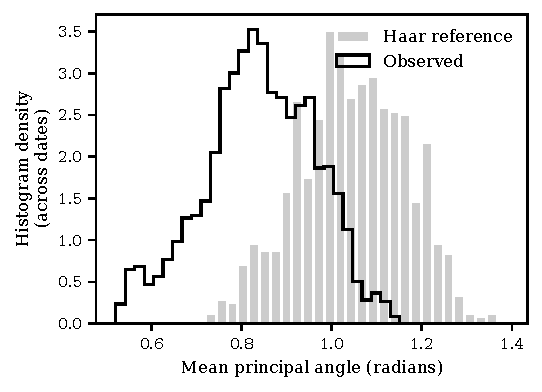
\includegraphics[width=0.72\linewidth]{figures/direction.pdf}
\caption{Histogram density across test dates for the mean principal angle. I show the Haar reference distribution and observed covariance-to-susceptibility angles ($n=\DirectionDateCount$ dates).}
\label{fig:directions}
\end{figure}

I report six distinct summaries rather than combining them into one score. Figure~\ref{fig:state} shows the test-period paths. $H$ stays close to the ten-dimensional ceiling and changes little; $R$ varies but has no stable surrogate-exceeding evidence. In this analysis, $H$ is near-constant and $R$ is noise-dominated, which undercuts H1's premise that these summaries provide a useful set of distinct state signals. This pattern is consistent with a near-identity, highly persistent fitted $J$ (median $\rho\approx0.99$), whose singular values are close.

\begin{figure}[!htbp]
\centering
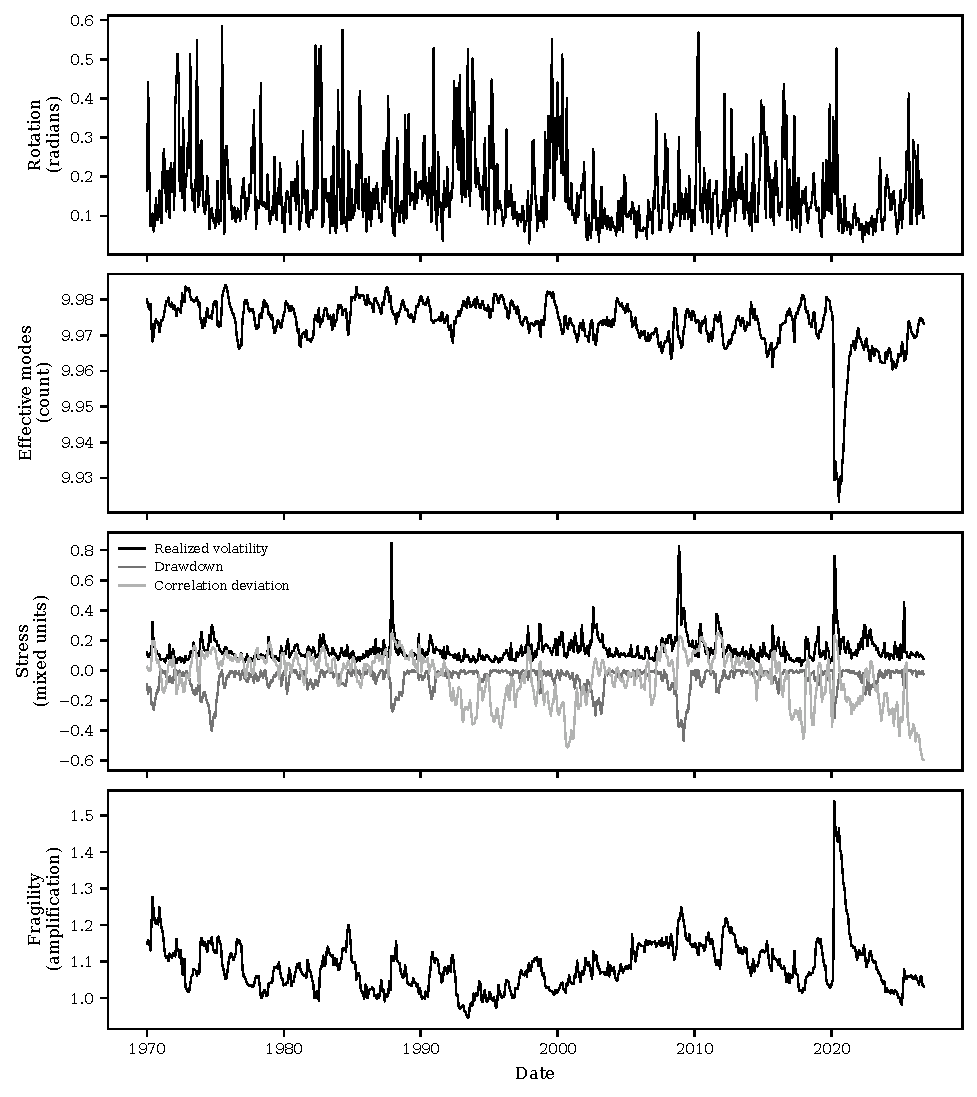
\includegraphics[width=0.84\linewidth]{figures/state.pdf}
\caption{The six components of $\mathbf M_t$ over the out-of-sample period. Volatility is annualized; drawdown and correlation deviation are unitless.}
\label{fig:state}
\end{figure}

\subsection{H1 signal and joint outcomes}
I find that only $F$ passes the adjusted block-shuffle test: $p_R=\HoneAdjpR$, $p_H=\HoneAdjpH$, and $p_F=\HoneAdjpF$. For the pre-onset placebo, I report raw and Holm-adjusted probabilities side by side: $R$ is $(\HoneEventRawpR,\HoneEventAdjpR)$, $H$ is $(\HoneEventRawpH,\HoneEventAdjpH)$, and $F$ is $(\HoneEventRawpF,\HoneEventAdjpF)$. Holm adjustment caps all three large raw values at one; I do not interpret these adjusted values as evidence that the observed statistics equal their placebo medians.

I find H1 \HoneVerdict{}. Condition (a) fails jointly because $R$ and $H$ do not meet the 0.01 surrogate threshold, although $F$ passes individually. Condition (b) fails because none of the adjusted pre-onset probabilities is below 0.05. Conditions (c) redundancy and (d) dimension pass. The frozen unsupported rule therefore does not apply, so the joint verdict remains inconclusive.

Table~\ref{tab:h1-conditions} gives the four frozen condition values and rules.

\begin{table}[!htbp]
\centering
\caption{Frozen H1 conditions and measured values. The pre-onset entries show raw/Holm-adjusted probabilities.}
\label{tab:h1-conditions}
\scriptsize
\begin{tabular}{@{}p{0.95in}p{2.55in}p{1.7in}l@{}}
\toprule
Condition & Frozen result & Rule & Outcome \\
\midrule
\HoneRows
\bottomrule
\end{tabular}
\end{table}

\begin{figure}[!htbp]
\centering
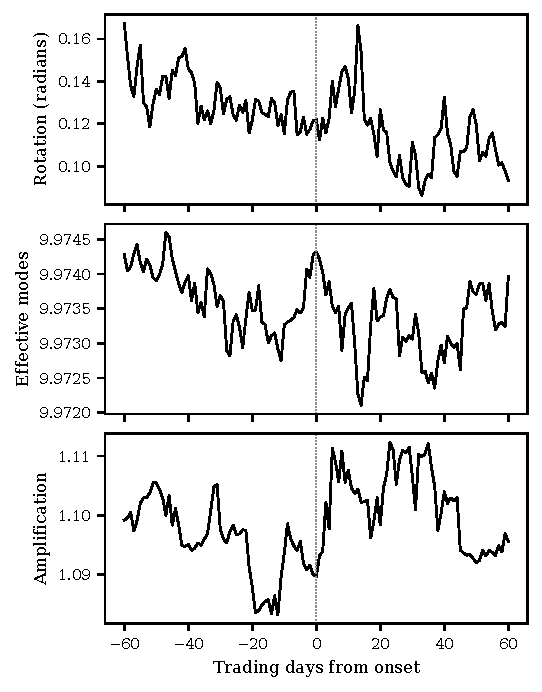
\includegraphics[width=0.72\linewidth]{figures/event_study.pdf}
\caption{Median rotation, entropy, and fragility around each test-period event onset. I use the date alignment descriptively; it does not establish causality.}
\label{fig:event}
\end{figure}

\subsection{H2 incremental prediction}
I find H2 \HtwoVerdict{}. Table~\ref{tab:h2} reports both frozen model comparisons. For the richer baseline, adding $F$ changes AUC by \DeltaMOne, with adjusted interval [$\DeltaMOneLow$, $\DeltaMOneHigh$]. Its point estimate is negative, and the adjusted upper bound is below the practical threshold of 0.02. The test contains \EventClusters{} event clusters and \AnchorCount{} common anchors.

In the post-freeze default forecast comparison, EWMA volatility alone reaches AUC $0.748$, at least as high as $M_1$ ($0.741$) and $M_1+F$ ($0.732$). In Table S4, at the $-10\%$ threshold and 60- and 120-session horizons, AUC falls below 0.5 for $M_1$, $M_1+F$, and EWMA. This may reflect the risk set: some high-volatility dates after an event can be labelled negative when no new onset falls within the forecast horizon. I treat this as a possible explanation, not a demonstrated cause.

\begin{table}[!htbp]
\centering
\caption{Frozen incremental out-of-sample AUC. An anchor is a risk date with an observed label and a prediction for each model in its comparison; I use the common anchors for each pair.}
\label{tab:h2}
\small
\begin{tabular}{@{}l>{\raggedright\arraybackslash}p{0.9in}>{\raggedright\arraybackslash}p{1.3in}lll@{}}
\toprule
Comparison & $\Delta$AUC & Adjusted interval & Holm $p$ & Clusters & Anchors \\
\midrule
\HtwoRows
\bottomrule
\end{tabular}
\end{table}

I see several plausible reasons why adding $F$ could lower AUC: it may overfit incremental variation when severe events are few; it may be collinear with stress already represented in $M_1$; or it may move too slowly to help a model fit on a small number of event clusters. These are explanations to test, not conclusions established by this comparison.

\begin{figure}[!htbp]
\centering
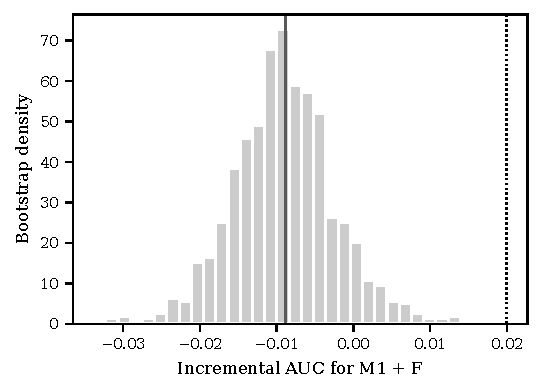
\includegraphics[width=0.72\linewidth]{figures/bootstrap.pdf}
\caption{Frozen block-bootstrap distribution of the richer-baseline AUC increment. I mark the point estimate and practical threshold.}
\label{fig:bootstrap}
\end{figure}

\FloatBarrier
\section{Post-freeze exploratory addendum}
After the protocol freeze, I wrote a separately hashed exploratory analysis plan and three separately hashed extensions, and I recorded each in the amendment log. I leave the primary analysis plan, protocol hash, and frozen study output unchanged. I use these additional analyses to assess sensitivity, not to revise the primary verdicts.

I count exact zero returns by estimation, calibration, and test period. I compare the frozen $10^{-8}$ floor with a $10^{-6}$ floor and with a filter treatment that skips the measurement update when a return is exactly zero. I keep zero source returns in the equal-weight target and stress series. I summarize the period counts and both reruns in the supplement.

For $F$, I rerun the primary, zero-treatment, subperiod, and forgetting-factor block-shuffle tests with \FPrecisionDraws{} draws per test. In the primary rerun, the observed median is \FPrimaryObserved{} versus a shuffled-null median of \FPrimaryNull{} (raw $p=\FPrimaryRawP$, Holm-adjusted $p=\FPrimaryHolmP$). The floor-$10^{-6}$ result is \FFloorObserved{} versus \FFloorNull{} (raw $p=\FFloorRawP$, Holm-adjusted $p=\FFloorHolmP$); with exact-zero observations treated as missing it is \FMissingObserved{} versus \FMissingNull{} (raw $p=\FMissingRawP$, Holm-adjusted $p=\FMissingHolmP$). The F surrogate result therefore depends on zero treatment: under the frozen $10^{-8}$ floor, $\log(0+c)=-18.42$ turns each exact zero into an extreme outlier. In both subperiods, the observed median is below the shuffled null: \FSubperiodSummary. The direction is lower amplification than shuffled data, not higher. These reruns show that $F$ survives under the frozen settings, but not under every alternative zero-handling or subperiod check.

I supplement the Haar comparison with a factor-aligned null that fixes the leading covariance direction and randomizes the remaining directions in its orthogonal complement. I report block-bootstrap uncertainty and an autocorrelation-adjusted effective sample size for both the frozen Haar percentile and the factor-aligned percentile. The factor-aligned result is less extreme: I obtain \FactorAlignedMedianPercentile, compared with \HaarMedianPercentile{} for the frozen Haar reference. This suggests that part of the apparent alignment reflects the market's leading factor. Across $\lambda\in\{0.990,0.995,0.998,0.999\}$, the post-freeze Holm-adjusted $F$ probabilities are \FLambdaHolmSummary. The median scale of $F$ depends on $\lambda$: it ranges from \FScaleLambdaRange, so the selected-setting median of 1.08 is not an absolute level. I find the entropy ceiling robust, but the scale of rotation sensitive to the forgetting factor.

For H2, I vary the drawdown threshold over $-10\%$, $-15\%$, and $-20\%$, the forecast horizon over 20, 60, and 120 sessions, and logistic $C$ over 0.1, 1, and 10. I report AUC levels and increments against a no-skill AUC of 0.5 and an EWMA-volatility-only baseline, along with precision and recall at a 5\% alert rate. A separate 399-replicate bootstrap resamples training blocks and refits the logistic models at the original expanding-window cutoffs; I hold the upstream filter and RLS path fixed. I also compare fixed-score interval bandwidths of 60, 125, and 250 sessions.

Across the 27 H2 settings, I estimate a positive AUC increment in six cases, but no point estimate reaches the 0.02 practical threshold. The upper interval remains below 0.02 in 20 settings; seven settings leave that threshold inside the interval. I report those less decisive cases rather than treating the frozen negative result as universal across target definitions.

For the frozen target and fitted scores, the fixed-score interval widens as the block length increases: I estimate intervals of $[-0.019,0.002]$, $[-0.020,0.003]$, and $[-0.021,0.005]$ for 60, 125, and 250 sessions. Each upper endpoint remains below 0.02.

I repeat the analysis on the 17-industry daily panel as an aggregation check. I match 19 of its 22 test clusters to ten-industry events within 120 sessions (86.4\%). Its raw $F$ surrogate probability is 0.002 from 499 draws, while the primary $F$ probability is Holm-adjusted after the 4,999-draw rerun; these values are not comparable. Adding $F$ changes H2 AUC by $-0.024$ (95\% interval $[-0.052,-0.001]$), which excludes zero and indicates that $F$ hurts on this panel, across 10,288 anchors. The heavy event overlap adds little independent H2 event power, so I do not treat this as a replication. I found no daily developed ex-U.S. industry series in the official French Library industry tables; its daily developed ex-U.S. portfolios are sorted by size and book-to-market, so I do not present them as an industry panel \cite{French}. I report the exploratory results and their hashes in the supplement.

\section{Discussion}
I draw a narrow conclusion from the frozen analysis: $F$ survives the block-shuffle null, but it does not add practical forecast value under H2. Entropy is near-constant and rotation is noise-dominated; both findings undercut H1's premise. $F$ survives under the frozen settings, but not under every alternative zero-handling or subperiod check. The post-freeze checks show how the result responds to zero treatment, null construction, event definition, model penalty, time period, forgetting factor, and portfolio aggregation; none alters the original joint verdict.

I interpret $F$ as a local sensitivity of a fitted response map. In future work, I could model a probability density over market states with a nonlinear drift and state-dependent diffusion, then use the Jacobian of the drift to describe local susceptibility. A nonlinear Fokker--Planck equation is one possible framework. I propose this only as a direction for later research; I do not estimate such a PDE here.

\section{Limitations}
\begin{itemize}
\item I use one U.S. historical return source and only 21 frozen test-period event clusters. The 17-industry check reaggregates largely the same stock universe and does not supply independent international event power.
\item My stress features omit funding, leverage, and liquidity. I forecast historical drawdowns and do not estimate a traded strategy or net performance.
\item My refit-aware bootstrap resamples logistic training and test blocks but holds the filtered state and RLS path fixed, so it does not include all upstream estimation uncertainty.
\item I disclose two access deviations: a final-row preview and pre-test data in an early lambda-selection harness. I saw no test-period aggregate or model result; I give the chronology in Supplementary Section~11.
\item The French Library can revise historical return files. I record snapshot hashes and provide a downloader, but an updated archive may not reproduce the frozen snapshot.
\end{itemize}

\section{Conclusion}
I find H1 inconclusive and H2 unsupported under the frozen decision rules. $F$ survives under the frozen settings, but not under every alternative zero-handling or subperiod check; adding it to the richer baseline does not achieve the prespecified practical AUC gain. Entropy stays near its ten-mode ceiling and rotation does not show robust surrogate evidence. The observed median $F$ is below the shuffled null, indicating less amplification than shuffled data. This audit therefore finds a setting-dependent local-sensitivity signal without evidence that it improves the selected drawdown forecasts.

\section*{Declarations}
\noindent\textbf{Funding.} I received no grant or external funding, and I did not seek funding for this project.\\
\textbf{Competing interests.} I disclose that I first designed Avarent as a proprietary algorithm product for quantitative funds and later decommissioned the Avarent project.\\
\textbf{AI assistance.} AI tools substantially assisted me with code, analysis scripts, and drafting. I developed the initial framework on paper and the C++ prototype, reviewed the code, analyses, and manuscript, and take responsibility for the reported methods and results.\\
\textbf{Data and code availability.} I obtained the ten-industry data from the \href{https://mba.tuck.dartmouth.edu/pages/faculty/ken.french/data_library.html}{Kenneth R. French Data Library} (archive retrieved \RetrievalDate) and the 17-industry daily panel from the same Library (retrieved \SecondaryRetrievalDate). I provide scripts that fetch both archives from the repository root. I do not redistribute the upstream French archives; their source terms apply. My code is available at \url{https://github.com/FFTryhard/Avarent}. I license code under MIT and my paper, figures, and derived results under \href{https://creativecommons.org/licenses/by/4.0/}{CC BY 4.0}. I list SHA-256 hashes for the source archives, derived panels, frozen study file, analysis plans, protocol, and executable in the supplement's reproducibility section.\\
\textbf{Disclaimer.} I do not provide investment advice and make no claim of trading performance.\\
\textbf{Acknowledgments and ethics.} I acknowledge the Kenneth R. French Data Library. I use public portfolio-level market data and no human-subject or individual-level records.

\FloatBarrier
\begin{thebibliography}{20}
\bibitem{Julier} Julier, S. J., and Uhlmann, J. K. (2004). Unscented filtering and nonlinear estimation. \emph{Proceedings of the IEEE}, 92(3), 401--422. doi:10.1109/JPROC.2003.823141.
\bibitem{HRS} Harvey, A. C., Ruiz, E., and Shephard, N. (1994). Multivariate stochastic variance models. \emph{The Review of Economic Studies}, 61(2), 247--264. doi:10.2307/2297980.
\bibitem{DavisKahan} Davis, C., and Kahan, W. M. (1970). The rotation of eigenvectors by a perturbation. III. \emph{SIAM Journal on Numerical Analysis}, 7(1), 1--46. doi:10.1137/0707001.
\bibitem{Wedin} Wedin, P.-A. (1972). Perturbation bounds in connection with singular value decomposition. \emph{BIT Numerical Mathematics}, 12(1), 99--111. doi:10.1007/BF01932678.
\bibitem{Kunsch} K\"unsch, H. R. (1989). The jackknife and the bootstrap for general stationary observations. \emph{The Annals of Statistics}, 17(3), 1217--1241. doi:10.1214/aos/1176347265.
\bibitem{Holm} Holm, S. (1979). A simple sequentially rejective multiple test procedure. \emph{Scandinavian Journal of Statistics}, 6(2), 65--70. doi:10.2307/4615733.
\bibitem{Roy} Roy, O., and Vetterli, M. (2007). The effective rank: a measure of effective dimensionality. In \emph{Proceedings of the 15th European Signal Processing Conference}, 606--610.
\bibitem{Kritzman} Kritzman, M., Li, Y., Page, S., and Rigobon, R. (2011). Principal components as a measure of systemic risk. \emph{The Journal of Portfolio Management}, 37(4), 112--126. doi:10.3905/jpm.2011.37.4.112.
\bibitem{Scheffer} Scheffer, M., et al. (2009). Early-warning signals for critical transitions. \emph{Nature}, 461(7260), 53--59. doi:10.1038/nature08227.
\bibitem{Hamilton} Hamilton, J. D. (1989). A new approach to the economic analysis of nonstationary time series and the business cycle. \emph{Econometrica}, 57(2), 357--384. doi:10.2307/1912559.
\bibitem{DichtlCrash} Dichtl, H., Drobetz, W., and Otto, T. (2023). Forecasting stock market crashes via machine learning. \emph{Journal of Financial Stability}, 65, 101099. doi:10.1016/j.jfs.2022.101099.
\bibitem{CoffmanNiederle} Coffman, L. C., and Niederle, M. (2015). Pre-analysis plans have limited upside, especially where replications are feasible. \emph{Journal of Economic Perspectives}, 29(3), 81--98. doi:10.1257/jep.29.3.81.
\bibitem{French} Kenneth R. French Data Library. Daily 10-industry and 17-industry portfolio returns. Retrieved \RetrievalDate{} and \SecondaryRetrievalDate. \url{https://mba.tuck.dartmouth.edu/pages/faculty/ken.french/data_library.html}.
\end{thebibliography}
\end{document}
